Refer to the bear growth data in Example 1.10 (see Table 1.4). Restrict your attention to
the measurements of length.
\begin{enumerate}[label=(\alph*)]
    \item Obtain the 95\% $T^{2}$ simultaneous confidence intervals for the four population means for length.
    
    \[
        \bar{\textbf{x}}
        =
        \begin{bNiceArray}{c}
            143.2857 \\
            159.2857 \\
            173.1429 \\
            177.1429
        \end{bNiceArray},
        \hspace{0.4cm}
        \textbf{S}
        =
        \begin{bNiceArray}{rrrr}
            15.2381 &  -8.9286 & -6.3810 &  -4.5476 \\
            -8.9286 &  99.9048 & -6.3810 & -54.2143 \\
            -6.3810 &  -6.3810 & 15.8095 &   1.4762 \\
            -4.5476 & -54.2143 &  1.4762 &  45.4762
        \end{bNiceArray}
    \]

    \[
        \bar{x}_{i}
        \pm
        \sqrt{
            \frac{(n-1)p}{(n-p)}
            F_{p, n-p}\left(\alpha\right)
        }
        \sqrt{
            \frac{s_{ii}}{n}
        }
    \]

    \[
        \begin{NiceArray}{rrrr}
            143.29 \pm \sqrt{72.94} \frac{\sqrt{15.24}}{\sqrt{7}} & \text{contains }\mu_{1} & \text{ or } & 130.69 \leq \mu_{1} \leq 155.89 \\
            159.29 \pm \sqrt{72.94} \frac{\sqrt{99.90}}{\sqrt{7}} & \text{contains }\mu_{2} & \text{ or } & 127.02 \leq \mu_{2} \leq 191.55 \\
            173.14 \pm \sqrt{72.94} \frac{\sqrt{15.81}}{\sqrt{7}} & \text{contains }\mu_{3} & \text{ or } & 160.31 \leq \mu_{3} \leq 185.98 \\
            177.14 \pm \sqrt{72.94} \frac{\sqrt{45.48}}{\sqrt{7}} & \text{contains }\mu_{4} & \text{ or } & 155.37 \leq \mu_{4} \leq 198.91
        \end{NiceArray}
    \]

    \item Refer to Part a. Obtain the 95\% $T^{2}$ simultaneous confidence intervals for the three successive yearly increases in mean length.
    
    \[
        \textbf{a}_{1}
        =
        \begin{bNiceArray}{r}
            -1 \\
             1 \\
             0 \\
             0
        \end{bNiceArray},
        \hspace*{0.2cm}
        \textbf{a}_{2}
        =
        \begin{bNiceArray}{r}
             0 \\
            -1 \\
             1 \\
             0
        \end{bNiceArray},
        \hspace*{0.2cm}
        \textbf{a}_{3}
        =
        \begin{bNiceArray}{r}
             0 \\
             0 \\
            -1 \\
             1
        \end{bNiceArray}
    \]
    so we can put them together into a matrix
    \[
        \textbf{A}
        =
        \begin{bNiceArray}{c}
            \textbf{a}_{2}^{\prime} \\
            \textbf{a}_{2}^{\prime} \\
            \textbf{a}_{3}^{\prime}
        \end{bNiceArray}
        =
        \begin{bNiceArray}{rrrr}
            -1 &  1 &  0 & 0 \\
             0 & -1 &  1 & 0 \\
             0 &  0 & -1 & 1
        \end{bNiceArray}
    \]
    With the matrix $\textbf{A}$ we can use Result 3.6 on page 144.

    The sample mean vector is
    \[
        \textbf{A}\bar{\textbf{x}}
        =
        \begin{bNiceArray}{rrrr}
            -1 &  1 &  0 & 0 \\
             0 & -1 &  1 & 0 \\
             0 &  0 & -1 & 1
        \end{bNiceArray}
        \begin{bNiceArray}{c}
            143.2857 \\
            159.2857 \\
            173.1429 \\
            177.1429
        \end{bNiceArray}
        =
    \]
    \[
        =
        \begin{bNiceArray}{r}
            -143.2857 + 159.2857 \\
            -159.2857 + 173.1429 \\
            -173.1429 + 177.1429
        \end{bNiceArray}
        =
        \begin{bNiceArray}{r}
            16      \\
            13.8571 \\
            4
        \end{bNiceArray}
    \]
    The sample covariance matrix is
    \[
        \textbf{A}\textbf{S}\textbf{A}^{\prime}
        =
    \]
    \begin{multline*}
        =
        \begin{bNiceArray}{rrrr}
            -1 &  1 &  0 & 0 \\
             0 & -1 &  1 & 0 \\
             0 &  0 & -1 & 1
        \end{bNiceArray}
        \begin{bNiceArray}{rrrr}
            15.2381 &  -8.9286 & -6.3810 &  -4.5476 \\
            -8.9286 &  99.9048 & -6.3810 & -54.2143 \\
            -6.3810 &  -6.3810 & 15.8095 &   1.4762 \\
            -4.5476 & -54.2143 &  1.4762 &  45.4762
        \end{bNiceArray} \\
        \times
        \begin{bNiceArray}{rrr}
            -1 &  0 &  0 \\
             1 & -1 &  0 \\
             0 &  1 & -1 \\
             0 &  0 &  1
        \end{bNiceArray}
        =
    \end{multline*}
    \[
        =
        \begin{bNiceArray}{rrr}
             133.0000 & -108.8333 & -49.6667 \\
            -108.8333 &  128.4762 &  33.5000 \\
             -49.6667 &   33.5000 &  58.3333
        \end{bNiceArray}
    \]

    \[
        \textbf{a}_{i}^{\prime}\bar{\textbf{x}}
        \pm
        \sqrt{
            \frac{(n-1)p}{(n-p)}
            F_{p, n-p}
            \left(\alpha\right)
            }
        \sqrt{
            \frac{
                \textbf{a}_{i}^{\prime}
                \textbf{S}
                \textbf{a}_{i}
                }{
                    n
                }
            }
    \]
    \[
        \begin{NiceArray}{rrrr}
            16.00 \pm \sqrt{72.94} \frac{\sqrt{133.00}}{\sqrt{7}} & \text{contains }\mu_{1} & \text{ or } & -21.23 \leq \mu_{1} \leq 53.23 \\
            13.86 \pm \sqrt{72.94} \frac{\sqrt{128.48}}{\sqrt{7}} & \text{contains }\mu_{2} & \text{ or } & -22.73 \leq \mu_{2} \leq 50.45 \\
            4.00 \pm \sqrt{72.94} \frac{\sqrt{58.33}}{\sqrt{7}} & \text{contains }\mu_{3} & \text{ or } & -20.65 \leq \mu_{3} \leq 28.65
        \end{NiceArray}
    \]

    \item Obtain the 95\% $T^{2}$ confidence ellipse for the mean increase in length from 2 to 3 years and the mean increase in length from 4 to 5 years.
    
    \begin{figure}[H]
        \centering
            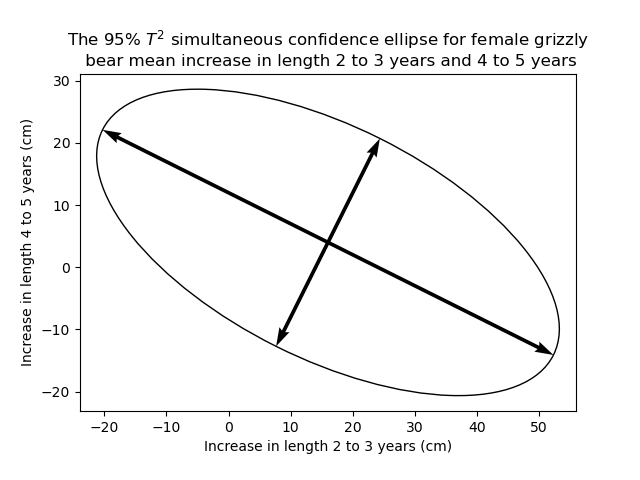
\includegraphics[scale=0.75]{./python/chapter-5/Question-5-10-c.png}
    \end{figure}
    
    \item Refer to Parts a and b. Construct the 95\% Bonferroni confidence intervals for the set consisting of four mean lengths and three successive yearly increases in mean length.
    
    We have two separate sets so we have two different values of $m$.

    For the first set consisting of four mean lengths, we have $m=4$ and
    $t_{n-1}\left(\frac{\alpha}{2m}\right) = t_{6}\left(\frac{0.05}{8}\right) = 3.52$, so
    \[
        \bar{x}_{i}
        \pm
        t_{n-1}
        \left(\frac{\alpha}{2m}\right)
        \sqrt{
            \frac{
                    s_{ii}
                }{
                    n
                }
            }
    \]

    \[
        \begin{NiceArray}{rrrr}
            143.29 \pm 3.52 \frac{\sqrt{15.24}}{\sqrt{7}} & \text{contains }\mu_{1} & \text{ or } & 138.09 \leq \mu_{1} \leq 148.48 \\
            159.29 \pm 3.52 \frac{\sqrt{99.90}}{\sqrt{7}} & \text{contains }\mu_{2} & \text{ or } & 145.98 \leq \mu_{2} \leq 172.59 \\
            173.14 \pm 3.52 \frac{\sqrt{15.81}}{\sqrt{7}} & \text{contains }\mu_{3} & \text{ or } & 167.85 \leq \mu_{3} \leq 178.43 \\
            177.14 \pm 3.52 \frac{\sqrt{45.48}}{\sqrt{7}} & \text{contains }\mu_{4} & \text{ or } & 168.17 \leq \mu_{4} \leq 186.12
        \end{NiceArray}
    \]
    For the second set consisting of three successive yearly increases in mean lengths, we have $m=p+3=4+3 = 7$ and
    $t_{n-1}\left(\frac{\alpha}{2m}\right) = t_{6}\left(\frac{0.05}{14}\right) = 4.00$, so

    \[
        \textbf{a}_{i}^{\prime}\bar{\textbf{x}}
        \pm
        t_{n-1}
        \left(\frac{\alpha}{2m}\right)
        \sqrt{
            \frac{
                \textbf{a}_{i}^{\prime}
                \textbf{S}
                \textbf{a}_{i}
                }{
                    n
                }
            }
    \]

    \[
        \begin{NiceArray}{rrrr}
            16.00 \pm 4.00 \frac{\sqrt{133.00}}{\sqrt{7}} & \text{contains }\mu_{1} & \text{ or } & -1.42 \leq \mu_{1} \leq 33.42 \\
            13.86 \pm 4.00 \frac{\sqrt{128.48}}{\sqrt{7}} & \text{contains }\mu_{2} & \text{ or } & -3.27 \leq \mu_{2} \leq 30.98 \\
            4.00 \pm 4.00 \frac{\sqrt{58.33}}{\sqrt{7}} & \text{contains }\mu_{3} & \text{ or } & -7.54 \leq \mu_{3} \leq 15.54
        \end{NiceArray}
    \]
    
    \item Refer to Parts c and d. Compare the 95\% Bonferroni confidence rectangle for the mean increase in length from 2 to 3 years and the mean increase in length from 4 to 5 years with the confidence ellipse produced by the $T^{2}$-procedure.
    
    \begin{figure}[H]
        \centering
            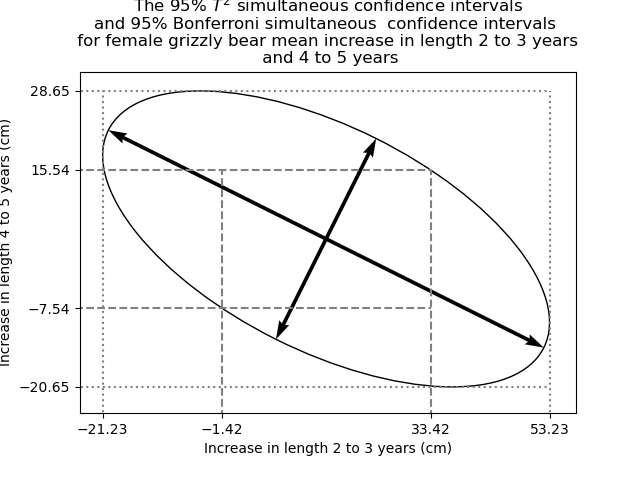
\includegraphics[scale=0.75]{./python/chapter-5/Question-5-10-e.png}
    \end{figure}
\end{enumerate}